% !TeX program = xelatex
% ============================================================
% passport_zh.tex - 太赫兹精密衰减器技术护照与校准证书
% ============================================================
\documentclass[11pt]{article}

\usepackage{myconfig}
\usepackage{booktabs}

% Overwrite main font to SimSun to support CJK Chinese characters and English
\setmainfont{SimSun}

% Reset figure numbering to sequential and translate captions to English/Chinese
\counterwithout{figure}{section}
\captionsetup[figure]{name=Figure, labelsep=period, font=small, labelfont=bf, justification=centering}

% Narrow fields locally to strictly fit everything on 2 pages
\geometry{
	left=1.4cm,
	right=1.4cm,
	top=1.0cm,
	bottom=1.0cm,
	headheight=0.4cm,
	footskip=0.4cm
}

% Tighten spacing around floats (figures/tables) to compress vertical size
\setlength{\floatsep}{4pt plus 2pt minus 1pt}
\setlength{\textfloatsep}{4pt plus 2pt minus 1pt}
\setlength{\intextsep}{4pt plus 2pt minus 1pt}
\setlength{\abovecaptionskip}{2pt plus 1pt minus 1pt}
\setlength{\belowcaptionskip}{2pt plus 1pt minus 1pt}

\singlespacing % Single line spacing for compact layout

\begin{document}
	\pagestyle{empty} % Remove page numbers for certificate template
	
	% ==========================================
	% PAGE 1: TITLE BLOCK & SPECIFICATIONS
	% ==========================================
	\noindent
	\begin{minipage}[c]{0.26\textwidth}
		\vspace{0pt}
		
\includegraphics[width=\textwidth]{tydex_logo}
	\end{minipage}
	\hfill
	\begin{minipage}[c]{0.72\textwidth}
		\vspace{0pt}
		\raggedleft
		{\large\bfseries Tydex LLC} \\
		{\small 光谱研究部门} \\
		\vspace{0.2em}
		{\color{headerblue}\large\bfseries 技术护照与校准证书} \\
		{\color{headerblue}\Large\bfseries 太赫兹可调精密衰减器} \\
		{\small 型号: \textbf{ATT-11-16-CA85} \quad | \quad 序列号: \textbf{\#02721}}
	\end{minipage}
	
	\vspace{0.3em}
	\hrule
	\vspace{0.3em}
	
	% Temporarily redefine footnote symbol to asterisk
	\renewcommand{\thefootnote}{*}
	
	\noindent
	\begin{minipage}[t]{0.81\textwidth}
		\vspace{0pt}
		\noindent\textbf{1. 应用与结构设计} \\
		\mycode{ATT-11-16-CA85} 太赫兹可调精密衰减器（通光孔径 85 mm）由两个独立的线栅偏振片组成。图1展示了太赫兹辐射穿过线栅 $P_1$ 和 $P_2$ 的实验装置示意图。第一个偏振片与入射光束的偏振方向一致（角度 $\theta_1 = 0^\circ$），而可旋转偏振片（检偏器）则旋转角度 $\theta_2 = \theta$。通过改变相对角度 $\theta = \theta_2 - \theta_1$ 来控制引入的衰减。该设备针对 0.05 至 2.0 THz（波长 $\lambda > 150$~$\mu$m）的频率范围进行了单独校准。
	\end{minipage}
	\hfill
	\begin{minipage}[t]{0.16\textwidth}
		\vspace{0pt}
		\centering
		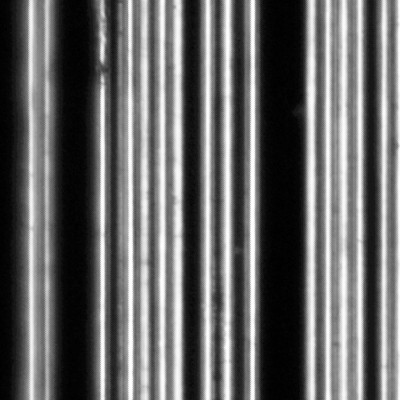
\includegraphics[width=\textwidth]{passport_microphoto}
		\par\vspace{1pt}
		{\small 线栅结构照片}
	\end{minipage}
	
	\vspace{0.3em}
	
	\noindent\textbf{2. 技术与校准规范}
	\begin{table}[H]
		\centering
		\small % Using small font size for table as per technical documentation standards
		\begin{tabularx}{\textwidth}{lX}
			\toprule
			\textbf{参数} & \textbf{数值 / 技术规范} \\
			\midrule
			通光孔径（夹具直径） & 85~mm \\
			标称线栅周期 $P$ / 金属丝直径 $D$ & $16.0$~$\mu$m / $11.0$~$\mu$m \\
			实测几何周期 $P_{\text{geom}}$（通过照片） & $15.93 \pm 5.03$~$\mu$m ($\pm 31.6\%$, 质量等级 "A") \\
			校准频率范围 & 0.05 -- 2.0 THz \\
			\midrule
			\textbf{Blanco 模型有效参数} & \textbf{用于校准曲线计算 (95\% 置信区间):} \\
			有效线栅周期 $P_{\text{eff}}$ & $15.50 \pm 0.05$~$\mu$m \\
			有效条带宽度 $D_{\text{eff}}$\footnotemark[1] & $5.67 \pm 0.08$~$\mu$m (消除漂移后的系综平均值) \\
			欧姆损耗因子 $loss\_factor$ & $0.368 \pm 0.045$ dB/THz$^{1.58}$ (幂律指数 $\gamma = 1.58$) \\
			系统角度偏差 $\theta_{\text{offset}}$ & $-0.45^\circ \pm 0.08^\circ$ (旋转台回程误差补偿) \\
			模型近似误差 (RMSE)\footnotemark[2] & $\pm 1.39$ dB (动态范围最大可达 $-45$ dB) \\
			\bottomrule
		\end{tabularx}
	\end{table}
	\footnotetext[1]{\scriptsize Blanco模型将圆柱形金属丝网映射为等效的扁平条带网。标称直径为 $D = 11.0$~$\mu$m 的圆导线与太赫兹辐射的电磁相互作用类似于宽度为 $d \approx D/2$ 的扁平金属条，从而得出较小的有效宽度 $D_{\text{eff}} \approx 5.67$~$\mu$m。损耗因子结合了幂律频率依赖性 $e^{-\alpha \nu^\gamma}$（其中 $\gamma=1.58$），以物理上描述从趋肤效应吸收（$\propto \nu^{0.5}$）到线栅边缘微小缺陷引起的瑞利散射（$\propto \nu^4$）的过程。参见：Blanco et al., \textit{Int. J. Infrared Millim. Waves}, vol. 7, no. 11, 1986.}
	\footnotetext[2]{\scriptsize 2D 残差分析表明，模型近似误差在很大程度上受大角度（$\theta > 50^\circ$）下未建模的多次线栅间反射和衍射散射的影响，而在小角度（$\theta < 45^\circ$）下局部拟合 RMSE 小于 $\pm 0.1$~dB。}
	
	\vspace{-0.5em}
	
	\noindent\textbf{3. 实验装置与测量方法} \\
	衰减器的校准是在 Menlo Tera K8 时域太赫兹光谱仪（THz-TDS）上进行的。入射太赫兹辐射具有水平线性偏振。图1展示了实验透射测量原理图。
	
	\begin{figure}[H]
		\centering
		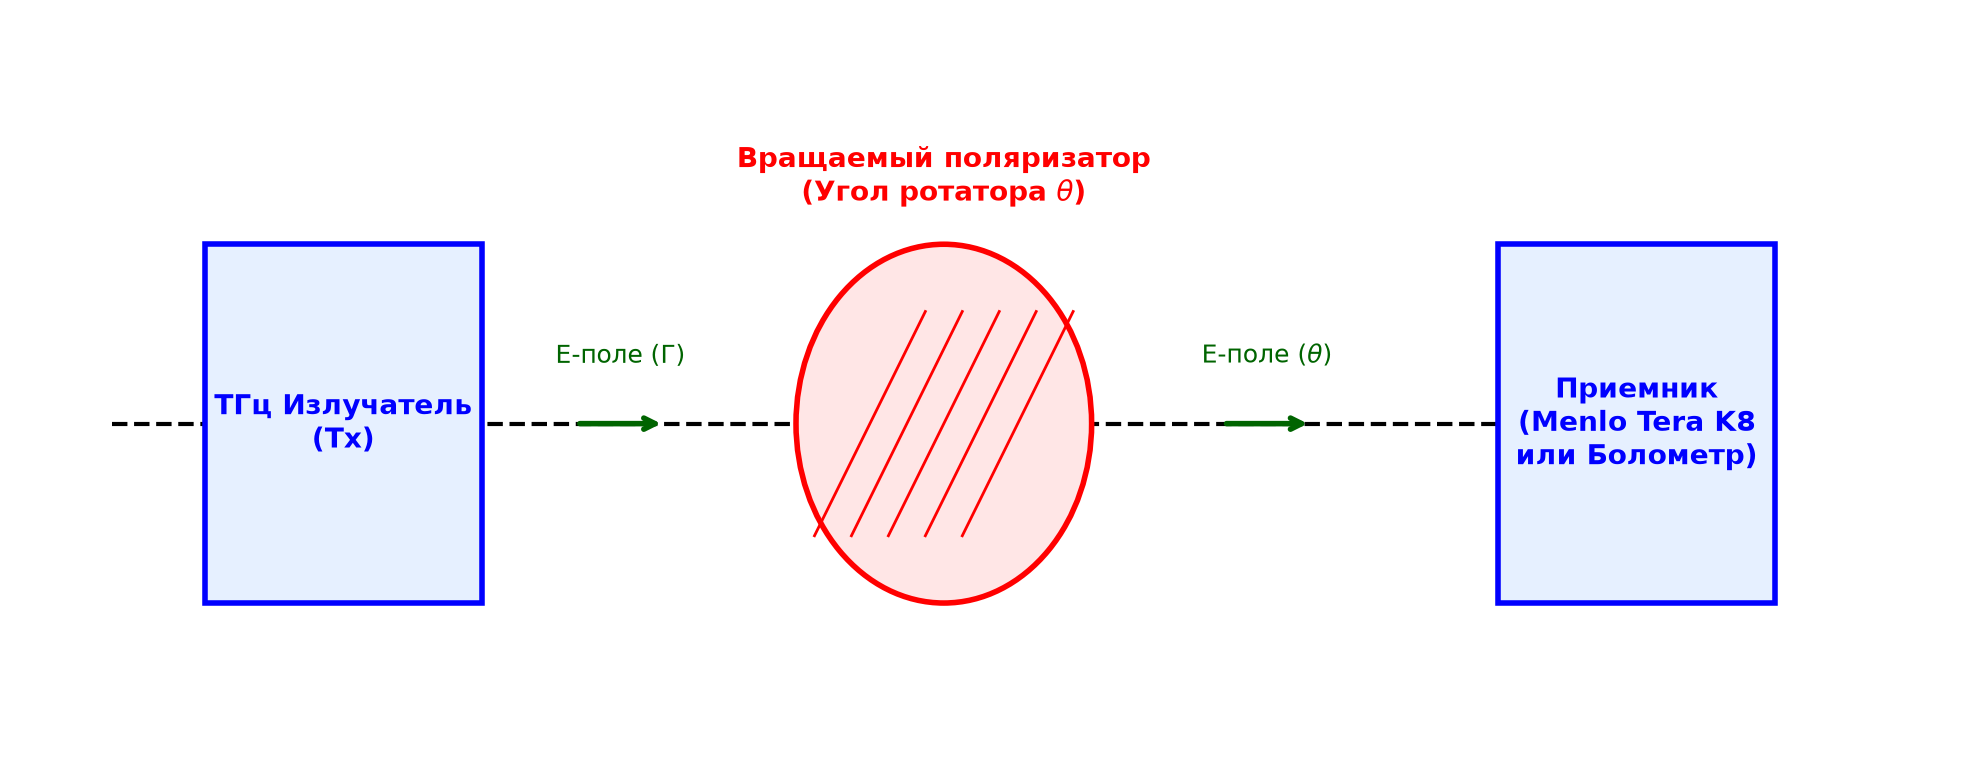
\includegraphics[width=0.48\textwidth]{fig0_1}
		\vspace{-0.5em}
		\caption{用于衰减器校准的实验装置示意图，其中偏振片角度为 $\theta_1$，检偏器角度为 $\theta_2$。}
		\label{fig:scheme}
	\end{figure}
	
	\newpage
	
	% ==========================================
	% PAGE 2: CALIBRATION CURVES & ERROR ANALYSIS
	% ==========================================
	\begin{center}
		{\color{headerblue}\large\bfseries 校准曲线与衰减误差分析}
	\end{center}
	
	\vspace{0.2em}
	
	\noindent\textbf{4. 衰减器应用场景} \\
	根据探测器类型，功率透射率 $T(\theta, \nu)$ 可通过 Blanco 模型\textsuperscript{*} 计算，其中 $t_{\perp}(\nu) = t_{\perp,0}(\nu) e^{-\frac{1}{2}\alpha \nu^{\gamma}}$ 和 $t_{\parallel}(\nu) = t_{\parallel,0}(\nu) e^{-\frac{1}{2}\alpha \nu^{\gamma}}$ 是经过损耗修正的复振幅透射系数（$t_{\perp,0}, t_{\parallel,0}$ 为纯电动力学 Blanco 系数，$\alpha = 0.0847$~Np/THz$^\gamma$，$\gamma = 1.58$），$\theta_{\text{offset}}$ 是系统角度偏差，而 $T_{\text{noise}}$ 是本底噪声：
	\begin{itemize}[leftmargin=0.6cm, itemsep=2pt, parsep=0pt, topsep=2pt]
		\item \textbf{场景 A} （PCA Menlo Tera K8 —— 光电导天线相干偏振敏感探测器）： \\
		$T(\theta, \nu) = \left| t_{\perp}(\nu) \cos^2(\theta - \theta_{\text{offset}}) + t_{\parallel}(\nu) \sin^2(\theta - \theta_{\text{offset}}) \right|^2 + T_{\text{noise}}$
		\item \textbf{场景 B} （辐射热测量计 / 戈莱池 —— 偏振不敏感探测器）： \\
		$T(\theta, \nu) = |t_{\perp}(\nu)|^2 \cos^2(\theta - \theta_{\text{offset}}) + |t_{\parallel}(\nu)|^2 \sin^2(\theta - \theta_{\text{offset}}) + T_{\text{noise}}$
	\end{itemize}
	
	\vspace{0.3em}
	
	\noindent\textbf{5. 校准透射率与衰减曲线} \\
	如需手动调整衰减，请使用图2中的图表曲线。要设置所需的衰减量 $A$（以 dB 为单位），在图2的垂直刻度（左侧或右侧）上找到目标值，并读取对应的旋转角度 $\theta$。左图显示了用于低衰减范围（$0^\circ - 60^\circ$）的线性透射刻度，而右图显示了用于高衰减范围（$30^\circ - 90^\circ$）的分贝刻度。图2中的 Menlo 实验数据点对应场景 A 的测量结果，证实了 Blanco 模型的高精度\textsuperscript{*}。
	
	\begin{figure}[H]
		\centering
		
\includegraphics[width=0.96\textwidth]{passport_calibration}
		\vspace{-0.5em}
		\caption{校准曲线：低衰减线性刻度（左）与高衰减分贝刻度（右）。右侧纵轴显示对应单位。}
		\label{fig:calib}
	\end{figure}
	
	\vspace{-0.5em}
	
	\noindent
	\begin{minipage}[t]{0.56\textwidth}
		\vspace{0pt}
		\noindent\textbf{6. 角度定位误差分析} \\
		由于马吕斯定律的三角函数特性，衰减量对旋转角度误差 $\Delta\theta$ 的敏感度在角度超过 $70^\circ$ 时会急剧上升。图3展示了在仪器机械回程误差分别为 $\Delta\theta = 0.5^\circ$ 和 $1.0^\circ$ 下场景 A 的衰减误差 $\Delta A$。
		
		\vspace{0.4em}
		\noindent\textbf{7. 计算软件与物理限制} \\
		供货清单中包含专用计算软件，用于计算任何频率 $\nu$ 和任意角度 $\theta$ 下的精确衰减。该软件基于有效参数 $P_{\text{eff}}$、$D_{\text{eff}}$ 和 $\theta_{\text{offset}}$，针对该特定设备（序列号：\#02721）进行了单独的校准。软件通过电子邮件进行分发。 \\
		\textit{物理限制}：在低于 10 GHz（波长 $\lambda > 3$ cm）的频率下，夹具的通光孔径（85 mm）将与波长处于同一数量级，会导致光束边缘产生衍射。
	\end{minipage}
	\hfill
	\begin{minipage}[t]{0.40\textwidth}
		\vspace{0pt}
		\centering
		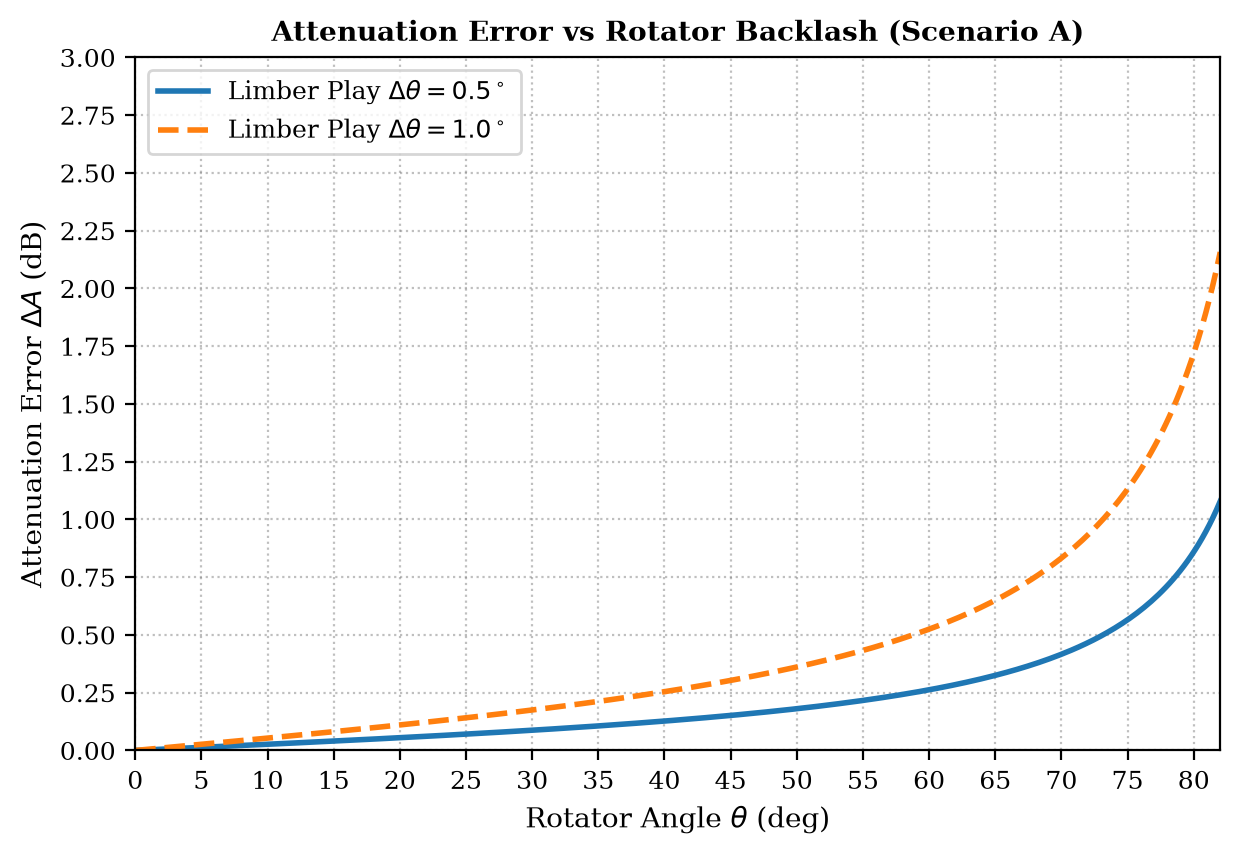
\includegraphics[width=\textwidth]{passport_error}
		\vspace{-0.6em}
		\captionof{figure}{在回程误差为 $\Delta\theta = 0.5^\circ$ 和 $1.0^\circ$（场景 A）下，衰减误差 $\Delta A$ 随旋转角度的变化曲线。}
		\label{fig:error}
	\end{minipage}
	
	\vspace{0.6em}
	\hrule
	\vspace{0.4em}
	\begin{center}
		\small
		校准日期：2026年6月29日 \\
		\vspace{0.3em}
		\textbf{Tydex有限责任公司 光谱研究部门} \hfill \textbf{操作员签名：\underline{\hspace{4cm}}}
	\end{center}
	
\end{document}
